% This is LLNCS.DEM the demonstration file of
% the LaTeX macro package from Springer-Verlag
% for Lecture Notes in Computer Science,
% version 2.4 for LaTeX2e as of 16. April 2010
% -
\documentclass{llncs}
% % % % % % % % % % % % % % % % % % % %
% For Russian uncomment the following lines
%\usepackage[utf8x]{inputenc}
 %\usepackage[russian]{babel}
% \def\keywordname{{\bf Ключевые слова:}}%
% % % % % % % % % % % % % % % % % % % % 
\usepackage{graphicx} 
\usepackage{comment}
\usepackage{xcolor}
\usepackage{epigraph}
\usepackage{amsmath}
\usepackage{amsfonts}
\usepackage{amssymb}
%\usepackage{natbib}
%\usepackage[title]{appendix}
\begin{document}
%


\title{Telling the story of best friends: marker rank statistics}
%
\titlerunning{Best friends}  
% abbreviated title (for running head)
%                                     also used for the TOC unless
%                                     \toctitle is used
%
\author{Alexander Favorov\inst{1}\textsuperscript,\inst{2}
\and Alexandra Suvorikova \inst{3}, Vera Mukhina \inst{2} \and Vasiliy Ramensky \inst{4}
\and Andrey Mironov \inst{5}}
%
\authorrunning{A. Favorov et al.} % abbreviated author list (for running head)
%
%%%% list of authors for the TOC (use if author list has to be modified)
\tocauthor{Alexander Favorov, Alexandra Suvorikova, Vera Mukhina, Vasiliy Ramensky, and Andrey Mironov}
%
\institute{
Johns Hopkins University School of Medicine, \\ Baltimore, MD 21205, USA,
\and
Vavilov Institute of General Genetics, RAS, \\ Moscow, 119333, Russia, 
\email{favorov@sensi.org}
\and
\textcolor{red}{Weierstrass institute, \\ Berlin, Germany,} 
\and
National Health and Research Center of Preventive Healthcare, \\ Moscow, 101990, Russia
\and
Faculty of Bioengineering and Bioinformatics, MSU, \\ Moscow, 119992, Russia
}

\maketitle              % typeset the title of the contribution

\renewcommand{\tag}{tag}
\newcommand{\cloud}{cloud}
\newcommand{\T}{T}
\newcommand{\C}{C}
\newcommand{\tl}{t}
\newcommand{\cl}{c}
%\setlength\epigraphwidth{.8\textwidth}
\setlength\epigraphrule{0pt}

\epigraph{SI AUGUSTUM VIDEAT AMICOS EIUS VIDEATI}

\vspace{-0.2in}

\begin{abstract}

\textcolor{green}{We define a tag's most friendly cloud as a cloud that pays maximal rank-normalized attention to the tag.}
\textcolor{blue}{ -- we will return here --} \textcolor{purple}{
Suppose we have a set of {\tag}s and a set of fuzzy set of {\tag}s, which we will refer to as {\cloud}s, and we have the {\tag}-to-{\cloud} relation quantified as a scalar for each $\left( {\tag},{\cloud}\right)$ pair. An example is: {\tag}s are genes, {\cloud}s are gene expression patterns, and the scalars are loads of the genes in the patterns. Sometimes, an observation that a gene is expressed implies the expression of a particular pattern (the simplest case is: the gene has nonzero load only in that pattern). If so, we say that the gene marks the pattern. Here we describe a statistical test that identifies pairs of a marker {\tag} and the marked {\cloud}. The test is based on rank statistics and it does not rely on propositions about the distribution of the relation quantity. The marked {\cloud} is referred to as the {\tag}'s best friend, and the test is named "the best friends test" or "the gene's best friends test". The statistics naturally expand to the case when a {\tag} selects (separates) a subset of {\cloud}s, thus having more than one best friend. The code (currently, only R) is available at \url{https://github.com/favorov/best-friends}
\keywords{best friends, gene's best friends, specific gene regulation, pattern marker, rank statistics, marker feature, marked entity}
}
\end{abstract}
%
\section{A simple intro: maybe abstract maybe frog}

There is a simple intuition of what it means to be a friend. A friend of Augustus cares about Augustus more than other people do. And, if we see Augustus, then we infer to see friends(s) of Augustus also. Let’s translate it into statistical language.

Consider a set of genes and their loads in a set of expression patterns. Each pattern represents a biological process by the expression levels of the involved genes. 

Sometimes, the expression of a single gene indicates the activity of the entire pattern. In the simplest case, the gene has a nonzero load in only one pattern. 
Moreover, the gene may have several nonzero loads, but all of them but one are relatively small. Then the gene (AKA Augustus) is the marker gene for the pattern, and the marked pattern is the best friend of this gene. We want to identify the marker genes and corresponding patterns statistically.  

\paragraph{Model} The bipartite graph naturally fits this model. To generalise the example, we will refer to genes as \textit{{\tag}s}, to expression patterns, as \textit{{\cloud}s}, and to any load as \textit{attention}. Fig.\ref{fig:nice_name} illustrates the setting.

\begin{figure}
    \centering
    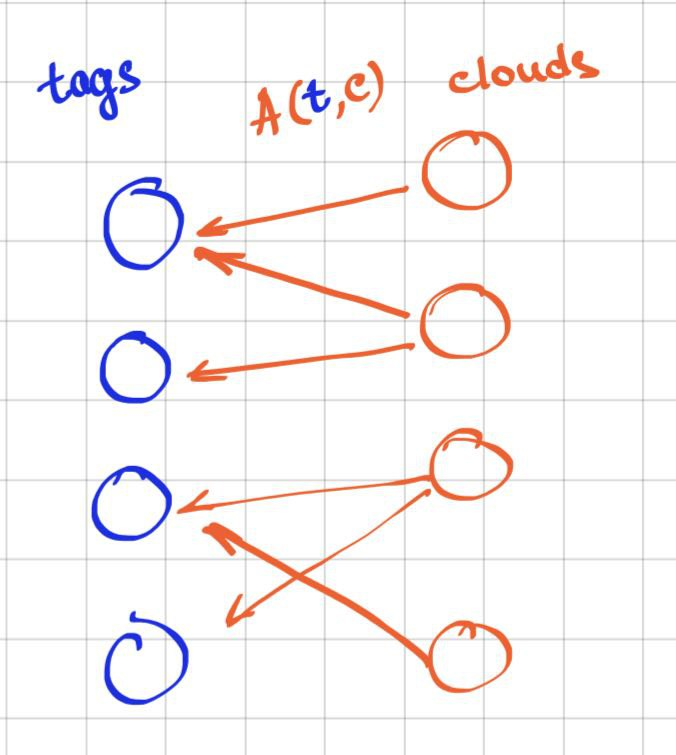
\includegraphics[scale=.25]{bipartite.jpg}
    \caption{The bipartite graph picture shows only edges with nonzero values.}
    \label{fig:nice_name}
\end{figure}

To be more specific, we are given a set of clouds $C = \{c_1, \dots, c_k\}$, and a set of tags $T = \{t_1, \dots, t_n\}$.
Each tag $t_i \in T$ and cloud $c_j \in C$ are related by the attention---the real value $a_{ij}$---that the cloud pays to the tag.
Let's agree that the greater the value, the higher the attention is. Naturally, the absence of attention corresponds to $a_{ij} = 0$. 

All the values $a_{ij}$ are stored in a matrix $\mathcal{A}$; its row $\mathcal{A}_{i:}$ corresponds to tag $t_i$, its column $\mathcal{A}_{:j}$ corresponds to cloud $c_j$.

This tag-cloud-attention metaphor applies to many problems in bioinformatics and statistics (see Tab.\ref{tab:examples} for examples).

\begin{table}[h!]
\centering
\begin{tabular}{c|c|c|c}
\textbf{Example} & \textbf{tag $t_i$} & \textbf{cloud $c_j$} & \textbf{attention $a_{ij}$} \\ 
\hline
\begin{tabular}[c]{@{}c@{}}gene regulation\\  by TFs\end{tabular}     & gene             & \begin{tabular}[c]{@{}c@{}}genes under \\ TF regulation\end{tabular}     & \begin{tabular}[c]{@{}c@{}}strength of \\ regulation\end{tabular}       \\ \hline
\begin{tabular}[c]{@{}c@{}}transcription \\ correlations\end{tabular} & gene             & \begin{tabular}[c]{@{}c@{}}genes coexpressed \\ with a gene\end{tabular} & \begin{tabular}[c]{@{}c@{}}transcription \\ correlation\end{tabular}    \\ \hline
fuzzy clustering                                                      & object           & cluster                                                                  & \begin{tabular}[c]{@{}c@{}}object weight \\ in cluster\end{tabular}     \\ \hline
\begin{tabular}[c]{@{}c@{}}transcription\\ decomposition\end{tabular} & transcript       & \begin{tabular}[c]{@{}c@{}}transcription \\ pattern\end{tabular}         & \begin{tabular}[c]{@{}c@{}}transcript's \\ load in pattern\end{tabular} \\ \hline

\begin{tabular}[c]{@{}c@{}}weighted graph\end{tabular} & vertex       & \begin{tabular}[c]{@{}c@{}} another vertex \end{tabular}         & \begin{tabular}[c]{@{}c@{}}weight of edge between\\ cloud and tag \end{tabular} \\ \hline
\end{tabular}

\caption{Tag-cloud metaphor deployment examples.}
\label{tab:examples}
\end{table}

\textcolor{red}{literature survey ctd here}

% \paragraph{Goal} 

%There is a simple intuition of what it means to be a friend. A friend of Augustus cares about Augustus more than about other people. And, if we see Augustus, then we infer to see friends(s) of Augustus also. Let’s translate it into statistical language.
% We remember that a friend of Augustus cares about Augustus more than about other people.



% \textcolor{purple}{For each tag, we want to identify the cloud(s) that particularly prefer(s) the tag, if any. Then such a cloud is a friend (or the best friend if there is only one) for the tag. The simplest example: imagine that only one cloud pays attention to the tag in hand. }

Let's recall the intuition that starts the introduction. A friend of Augustus cares about Augustus more than other people do. 

We express how much a cloud $c_j$ cares about a tag $t_i$ in terms of the rank of $a_{ij}$ in column $\mathcal{A}_{:j}$. So, if a cloud $c_j$ cares about a tag $t_i$ more than other clouds, the rank of $a_{ij}$ in $\mathcal{A}_{:j}$ is higher than the rank of $a_{il}$ in $\mathcal{A}_{:l}$ for all $l \neq j$. 

A question naturally arises: whether $c_j$ is a real best friend of $t_i$ or $c_j$ appeared at the top of the ranking just because there is always something at the top.

 
% To identify the friend(s), first, for each cloud, we rank all the tags by the attention the cloud pays to the tag. The ranking the decreasing, the first is the best. In other words, we create the rank matrix $\mathcal{R}$ of the same $|T|x|C|$ size, and each element is the corresponding attention's rank inside inside the column of the attention matrix. We normalise the values to be in $[0,1]$ by dividing by $|T|$ and we refer to the normalised ranks as $r$ matrix. Now, for each tag, we define the degree of friendliness of a cloud for this tag, by ranking the tag's row in $r_{i,j}=r(t_i,c_j)$ matrix. The most friendly cloud $c_{(1)}(t_i)$ is the cloud with the minimal value of $R_{ij}$, the next is $c_{(2)}(t_i)$, etc, etc.    

% 
%For a similar test that splits all the clouds into $m$ friends of the tag and the remaining $|C|-k$ clouds uses the difference  $r(t_i,c_{(m+1)}(t_i))$ and $r(t_i,c_{(m)}(t_i))$. If we obtain the p-value that is small enough, we claim that the clouds $c_{(1)}(t_i)$..$c_{(m)}(t_i)$ are friends of $t_i$ and $t_i$ is their marker.



%\paragraph{Statistical test} 

%We intend to express the meaning of the word "particularly" in this context by a statistical test.
 
We intend to statistically validate the hypothesis about true friends. 

Under $H_0$ we assume that there is no particular preferences between clouds and tags.
In other words, all the $n \times k$ attention values from clouds to tags are independent. Moreover, all the $n$ attention \textcolor{red}{values} that a cloud pays to tags are identically distributed.

\begin{itemize}
    \item Requires only $\mathcal{A}$
    \item What happens under $H_0$?
    \item Solution: Ranking of elements in $\mathcal{A}$ (rank-based)
    \item Thus, distribution-free
\end{itemize}



%Here we describe a statistical test that identifies pairs of a marker {\tag} and the marked {\cloud}. 
The test is distribution-free and based on rank statistics. 
%and it does not rely on propositions about the distribution of the relation quantity. 






\textcolor{violet}{The marked {\cloud} is referred to as the {\tag}'s best friend and the test is named "the best friends test" or "the gene's best friends test". The statistics naturally expand to the case when a {\tag} selects (separates) a subset of {\cloud}s, thus having more than one best friend.}


%We formulated \cite{best_friends:2015} the similar task in a symmetric form on gene expression data as searching for genes that are best friends of genes. Best friend of a gene $G_i$ is another gene $G_j$ that is expressed concertedly with the gene $G_i$, while other genes $G_k, k\neq i, k \neq j$ are (almost) not. The best friend is unique, while one gene can be the best friend for more than one gene. The solution we proposed (rank backwards ranking) showed the putative pairs of marker and its best friend, but it did not provide either statistical measure or an effect size estimate. Later, the problem was also formulated in an asymmetric setup \cite{patternmarkers:2017} for genes and expression patterns, and the solution was to scale each gene's loads to $max((\mbox{all loads for this gene})==1$ and calculate the Euclidean distance between the scaled vector of loads and the ideal $(0,0,...,1,...0$). The less the distance is, the better the marker is. 

%\textcolor{red}{literature survey ctd here}


%=======
%The measures of proximity in a network that aggregates knowledge about the distance of more than two elements are in the focus of applied math. as far as their current computational power allows to create 







 
% and a set . Each tag can be related to each cloud, and the strength of the relation varies from one (tag,cloud) pair to another. We refer to the relation strength as the attention that a cloud pays to a tag. The attention that each cloud pays to each tag is represented by a real value and is described by a scalar function $A(t, c)$. Some examples are presented in the table below.

%Let $T = \{t_1, \dots, t_n\}$ be a fixed set of tags. We assume, that there is a set of $k$ entities (referred to as clouds) $C = \{c_1, \dots, c_k\}$ paying attention on each of the tags. 


%-------------------
% The attention actually can be any type of relation measure, e.g. fuzzy membership. The absence of the attention is supposed to be represented by the smallest value, naturally, it is 0 and all the attention values are are positive (not required). The attention values are stored in $n\times k$ matrix $\mathcal{A}$.

% The tag-cloud-attention metaphor allows to represent a lot of applications in bioinformatics and statistics. The examples are gene patterns (cloud) and genes (tags) loads (attention) in the patterns; fuzzy sets (clouds, their elements (tags) and the inclusion degree (attention); weighted graph vertices (tags) and each vertex neighbourhood (cloud), here the attention is the weight of the edge.

%-------------- содержательная часть 
% Now, the question. For each tag, we want to identify the cloud(s) that specifically prefer(s) the tag. We say that such a cloud is a friend (or the best friend if it the the only) for the tag. The simplest example: imagine that only one cloud pays attention to our tag. 

% To identify the friend(s), first, for each cloud, we rank all the tags by the attention the cloud pays to the tag. The ranking the decreasing, the first is the best. In other words, we create the rank matrix $\mathcal{R}$ of the same $|T|x|C|$ size, and each element is the corresponding attention's rank inside inside the column of the attention matrix. We normalise the values to be in $[0,1]$ by dividing by $|T|$ and we refer to the normalised ranks as $r$ matrix. Now, for each tag, we define the degree of friendliness of a cloud for this tag, by ranking the tag's row in $r_{i,j}=r(t_i,c_j)$ matrix. The most friendly cloud $c_{(1)}(t_i)$ is the cloud with the minimal value of $R_{ij}$, the next is $c_{(2)}(t_i)$, etc, etc.    

% 
%For a similar test that splits all the clouds into $m$ friends of the tag and the remaining $|C|-k$ clouds uses the difference  $r(t_i,c_{(m+1)}(t_i))$ and $r(t_i,c_{(m)}(t_i))$. If we obtain the p-value that is small enough, we claim that the clouds $c_{(1)}(t_i)$..$c_{(m)}(t_i)$ are friends of $t_i$ and $t_i$ is their marker.




%\section{Introduction: friends and markers}

% There is a simple intuition of what does it mean to be a friend. A friend of Augustus cares about Augustus more than about other persons. And, if one sees Augustus, it makes sense to infer to see friends(s) of Augustus also. Lets’s try to translate it to statistical inferences.

% Let's picture a set of genes and their loads in expression patterns. Each pattern describes the expression of the genes in some process. Sometimes, we can conclude that a pattern is expressed from expression of a single gene. The simplest case that allows this inference is when the gene has nonzero load in only one pattern. The situation when other loads are just relatively small, also fits the inference. We will refer to the gene as marker gene and to the pattern as the best friend of the gene. We want to identify the marker genes and their best friends given the load matrix.

% We formulated \cite{best_friends:2015} the similar task in a symmetric form on gene expression data as searching for genes that are best friends of genes. Best friend of a gene $G_i$ is another gene $G_j$ that is expressed concertedly with the gene $G_i$, while other genes $G_k, k\neq i, k \neq j$ are (almost) not. The best friend is unique, while one gene can be the best friend for more than one gene. The solution we proposed (rank backwards ranking) showed the putative pairs of marker and its best friend, but it did not provide either statistical measure or an effect size estimate. Later, the problem was also formulated in an asymmetric setup \cite{patternmarkers:2017} for genes and expression patterns, and the solution was to scale each gene's loads to $max((\mbox{all loads for this gene})==1$ and calculate the Euclidean distance between the scaled vector of loads and the ideal $(0,0,...,1,...0$). The less the distance is, the better the marker is. 

% \textcolor{orange}{Let's make a generalisation. We have entities and features and a matrix that show how strong is a feature ascribed to an entity. We want to identify those features that reliably and uniquely identify an entity. Let's call the feature the entity's marker and let's call the entity the feature's best friend. Here, we describe a rank test identifying significant pairs of marker features and the corresponding best friends.}



%
\section{Method}
\label{sec:method}
The attention matrix $\mathcal{A}$ (see above) is the only input for the statistical test. Each its elements $a_{ij}$ is the strength of attention that a cloud $c_j \in C$
 pays to a tag $t_i \in T$
\[
\mathcal{A} = \begin{pmatrix}
a_{11} & a_{12} & \dots & a_{1k} \\
       &\cdots & \cdots &  \\
a_{n1} & a_{n2} & \dots & a_{nk}
\end{pmatrix}.
\]
%~\text{for all}~i \in \{1, \dots, n\}, j  \in \{1, \dots, k\}
Each column in $\mathcal{A}$ ($\mathcal{A}_{:j} =(a_{1j}, \dots a_{nj})'$ with $'$ denoting transposition)  stores the information about the strength of attention that the cloud $c_j$ pays to each tag in $T$. 

%Under $H_0$ we assume all values in $\mathcal{A}$ are independent. Moreover, the values in each $\mathcal{A}_{:j}$ are i.i.d.
%In what follows, we consider separately the case of symmetric $\mathcal{A}$.

For each cloud $c_j \in C$ we rank the elements inside
$\mathcal{A}_{:j}$.
Namely, we decreasingly order $\mathcal{A}_{:j}$. So for each $a_{ij} \in \mathcal{A}_{:j}$, we have the ordinal number $R_{ij}:=\text{rank}\left(a_{ij}|\text{inside}~\mathcal{A}_{:j}\right)$. We resolve ties by the mean rank of the tied elements. 

Let's denote the rank matrix as 
\[
\mathcal{R} = \begin{pmatrix}
R_{11} & R_{12} & \dots & R_{1k} \\
       &\cdots & \cdots &  \\
R_{n1} & R_{n2} & \dots & R_{nk}
\end{pmatrix}, 
\]
and its $i$-th row as $\mathcal{R}_{i:} = (R_{i1}, \dots, R_{ik})$.

To quantitatively express friendliness, we order the attention ranks to the same tag $t_i$ from different clouds. In our notations, it means we decreasingly order elements in $\mathcal{R}_{i:}$.

Let's denote the cloud-index of the smallest entry in $\mathcal{R}_{i:}$ as $\sigma_i(1)$, the cloud-index of the second smallest entry as ${\sigma_i(2)}$, etc. 

We refer to the corresponding clouds as $c_{i(1)}$, $c_{i(2)}$, etc. This notation is in accordance with that accepted in rank statistics applications \cite{Gut:2009}. 
So, the most friendly cloud for the tag $t_i$ is $c_{i(1)}$.
 

\textcolor{violet}{For a cloud to be a tag's best friend it is \textit{necessary} to be the most friendly cloud for the tag, but it is \textit{not enough}. Indeed, in any ranking, there is the first element. Our goal is to statistically estimate whether the most friendly tag is the most friendly by chance.} 


\textcolor{violet}{In other words, the attentions $A(t_i, c_j)$ that a cloud $c_j$ pays to all the tags $t_i$ are independently sampled from the same distribution. The attentions from different clouds to all the tags are also independently sampled. At the same time, they can be sampled from different distributions.}


\textcolor{red}{Explain $H_1$!}
\textcolor{purple}{The idea of $H_1$ is that...}

To statistically infer whether the most friendly cloud for the tag $t_i$ is really the best friend, we use the difference $R_{1\sigma(1)} - R_{1\sigma(2)}$,
%, in other words, between the next-after-the-best and the best values $r$ for the tag $t_i$.
\[
u(t_i) := \frac{R_{i\sigma(1)} -  R_{i\sigma(2)}}{n}.
\]
We explain the $n$-normalization in more detail in Section \textcolor{red}{...}.
%$, and all the elements inside the row $\mathcal{R}_{i:}$ are independent if the null hypothesis holds.

As a statistical test we use the $p$-value of $u(t_i)$, 
\[
P\left(u(t_i) \ge ... \right)
\]



We estimate the probability (p-value) to observe this difference as $\leq q$ given the null hypothesis proposition. If p-value is small enough, we reject the null, and claim that the friendliness of the cloud $c_{(1)}(t_i)$ is unlikely to observe by random and so we refer to it as the best friend of $t_i$. In this case, $t_i$ is a marker of its best friend cloud $c_{(1)}(t_i)$.


\textcolor{purple}{ 
%If a cloud is the tag's best friend, it is to be the most friendly cloud for the tag. The condition is necessary, but not enough. Indeed, in any ranking, there is a first element, and we want to estimate the probability to observe what we observe by random.
% The null hypothesis we use to picture a random setup is that in any column of $\mathcal{R}$ all the elements are i.i.d., or, in other words, the attention that a cloud pays to all the tags are independently sampled from the same distribution. The distributions can differ from cloud to cloud. 
|%The statistics we use to test whether the most friendly cloud for the tag $t_i$ is really the best friend is the difference $t$ between the values $r(t_i,c_{(2)}(t_i))$ and $r(t_i,c_{(1)}(t_i))$, in other words, between the next-after-the-best and the best values $r$ for the tag $t_i$.
% We estimate the probability (p-value) to observe this difference as $<=t$ given the null hypothesis proposition. If p-value is small enough, we reject the null, and claim that the friendliness of the cloud $c_{(1)}(t_i)$ is unlikely to observe by random and so we refer to it as the best friend of $t_i$. In this case, $t_i$ is a marker of its best friend cloud $c_{(1)}(t_i)$.
}
%Since we will apply this procedure for each tag $t_i\in T$, we slightly change the notations and denote 
% \[
% r_{i(q)} = r_{(q)}(t_i)...
% \]

%We will denote the corresponding cloud $c_{(1)}(t_i)$

\textcolor{purple}{
 To identify the friend(s), first, for each cloud, we rank all the tags by the attention the cloud pays to the tag. The ranking the decreasing, the first is the best. Then the corresponding ranks $r(t_i,c_j)$ are stored in the $n\times k$ matrix $\mathbb{R}$. Now, for each tag, we define the degree of the friendliness of a cloud for this tag, by ranking the tag's row in $\mathbb{R}$ matrix. The most friendly cloud $c_{(1)}(t_i)$ is the cloud with the minimal value of $R_{ij}$, the next is $c_{(2)}(t_i)$, etc, etc. 
If a cloud is the best friend, it is to be the most friendly cloud for the tag, but it is not enough. In any ranking, there is a first element, and we want to estimate the probability to observe what we observe by random. The null hypothesis we use to picture a random setup is that in any column of $\mathcal{R}$ all the elements are i.i.d., in other words, attentions that a cloud pays to all the tags are independently sampled from the same distribution. The distributions can differ from cloud to cloud. 
The statistics we use to test, whether the most friendly cloud for the tag $t_i$ is really the best friend, is the difference $\Delta$ between the values $r(t_i,c_{(2)}(t_i))$ and $r(t_i,c_{(1)}(t_i))$. We estimate the probability (p-value) to observe this difference as $\leq \Delta$ given the null hypothesis proposition. If the p-value is small enough, we reject the null and claim that the friendliness of the cloud $c_{(1)}(t_i)$ is unlikely to observe by random and so we refer to it as the best friend of $t_i$. In this case, $t_i$ is a marker of its best friend cloud $c_{(1)}(t_i)$.
For a similar test that splits all the clouds into $m$ friends of the tag and the remaining $n-k$ clouds uses the difference  $r(t_i,c_{(m+1)}(t_i))$ and $r(t_i,c_{(m)}(t_i))$. If we obtain the p-value that is small enough, we claim that the clouds $c_{(1)}(t_i), \dots, c_{(m)}(t_i)$ are friends of $t_i$ and $t_i$ is their marker.}

%%%------



% Now, for each tag, we define the degree of the friendliness of a cloud for this tag, by ranking the tag's row $\mathcal{R}_{i:}= \{r_{i1}, \dots, r_{ik}\}$. 

% The most friendly cloud $c_{(1)}(t_i)$ is the cloud with the minimal value of $R_{ij}$, the next is $c_{(2)}(t_i)$, etc, etc. 
% \[
% c_{(q)}(t_i) = c_{j}, \quad \text{where}~j~\text{is such that}~ q = \text{rank}(r_{ij}|\text{inside}~\mathcal{R}_{i:}).
% \]









% \textbf{Step 1. Find the tag's friend(s) among the clouds} We rank all the tags by the attention the cloud pays to the tag. 
% For each $t$ in $T$ and each $c$ in $C$, we describe the intensity of attention $c$ pays to $t$ as a scalar function $A(t, c)$. 
% Let $A(t, c)$ to be known for all $t\in T$ and all $c \in C$. This information about attention is stored in the matrix of size $n\times k$, \textit{i.e.}, for all $i \in \{1, \dots, n\}, j  \in \{1, \dots, k\}$:
% \[
% \mathcal{A} = (a_{ij}), 
% \quad a_{ij} = A(\tl_i, \cl_j).
% \]
% In other words, $j$-th column in $\mathcal{A}$ contains the information about the intensity of attention which the cloud $c_j$ pays to all tags in $T$,
% we denote it as 
% $\mathcal{A}_{:j} =(a_{1j}, \dots a_{nj})$.
% The ranking the decreasing, the first is the best. 


% Now we create the rank matrix $\mathcal{R}$ of the same $n\times k$ size, and each element is the corresponding attention's rank inside the column of the attention matrix. %We normalise the values to be in $[0,1]$ by dividing by $n$ and we refer to the normalised ranks as $\mathcal{R}$ matrix as well.

% \textcolor{red}{The method described below identifies the most friendly cloud for each tag $\tl_i$. Comment: the most friendly chuvak is a putative best friend.}
% To do this, we decreasingly order $\mathcal{A}_{j}$, and thus for each $a_{ij}$ we find the ordinal number 
% $R_{ij} := \text{rank}(a_{ij}|\text{inside}~\mathcal{A}_{:j})$.
% Of note, we resolve ties by the mean rank of the tied elements.

% The next step is to store all $r_{ij}$ the new matrix,
% \[
% \mathcal{R} = (r_{ij}), \quad \text{with}~ r_{ij} = \frac{R_{ij}}{n}.
% \]
% It contains the ranks of the tags inside the clouds. One may interpret $\mathcal{R}$ as the rank-normalized intensity of the attention that the clouds pay to the tags.






%(they come from the same distribution).

%\subsection{Asymmetric $\mathcal{A}$}

%In case of asymmetric $\mathcal{A}$ the ...

%\subsection{Symmetric $\mathcal{A}$}
\section{Statistical test}

\textcolor{blue}{Mapping huiapping} \cite{Solomon2018OptimalTO}

Let's denote
\[
r_{ij} = \frac{R_{ij} - \frac{1}{2}}{n}.
\]
In other words, each $r_{ij}$ is the normalized rank of the attention $A(t_i, c_j)$ inside $\mathcal{A}_{:j}$. 

We will explain this particular choice of rank normalization in Section~\textcolor{red}{...}.

By construction, all the elements of $\mathcal{R}$ are uniformly distributed and independent.


\subsection{Single marker rank statistics}

% +\subsection{Multiple marker rank statistics}



%============
For each feature (tag!) $i,i=1\dots k$, we obtain a vector $r_{ij}, j=1..n$. There are normalised ranks of the feature in different entities, in the a null hypothesis they are uniformly i.i.d. in [0,1]. Let's create a rank statistics $u_i$ by ordering their values. If a feature is a unique marker for an entity, the entity corresponds to the first  value $u_1$. Let's use the difference $u_2-u_1$ as a measure of uniqueness (quality of the marker). Indeed, if we see that the difference is significantly higher than we can expect if null hypothesis holds, we can conclude that the feature unexpectedly prefer the entity, so it is a marker (and the entity is its best friend). Similarly to the density estimation for each $u_i$ (see, e.g. \cite{Gut:2009}) we estimate the probability to observe the difference $u_2 - u_1 \ge t$. 

First, the whole n-dimension (nD) volume of ranked variables $u_1 .. u_n$ is:
\begin{eqnarray*}
V = &\displaystyle \int_0^1\int_{u_1}^1\int_{u_2}^1\int_{u_3}^1...\int_{u_{n-1}}^1 du_n....du_4 du_3 du_2 du_1 =  \frac{1}{n!}
\end{eqnarray*}
see eq. \ref{eq:volume} for details.

Let's denote the p-value for the observation $t=u_2-u_1$ as $p_1(t)$. $p_1(t)$ is the ratio of the nD volume, that is limited by $t<=u_2-u_1$ condition, and $V$.

\begin{eqnarray*}
p(t) = & \displaystyle\frac{1}{V} \displaystyle \int_0^{1-t}\int_{{u_1}+t}^1\int_{u_2}^1\int_{u_3}^1...\int_{u_{n-1}}^1 du_n....du_4 du_3 du_2 du_1 = (1-t)^n
\end{eqnarray*}
see eq. \ref{eq:p_1} for details.

After the correction this p-value for multiple hypothesis testing (each feature provides its own null hypothesis), we identify the statistically significant pairs of a feature (marker) and entity (its best friend).

\subsection{Multiple marker rank statistics}
Now, let's suppose that an entity has more than one features, that almost equally good marks it, for example, two genes has nonzero load in a pattern. The pattern is the best friend for both of them, and each of them or their combination is a unique marker for the pattern, but the single marker rank statistics cannot find them, for the distance $u_2-u_1$ is quite low: the markers are almost equally good.

\section*{Notes and comments}

For a symmetric case, sometimes it makes sense to remove the main diagonal before ranking not to obtain trivial self-relations.

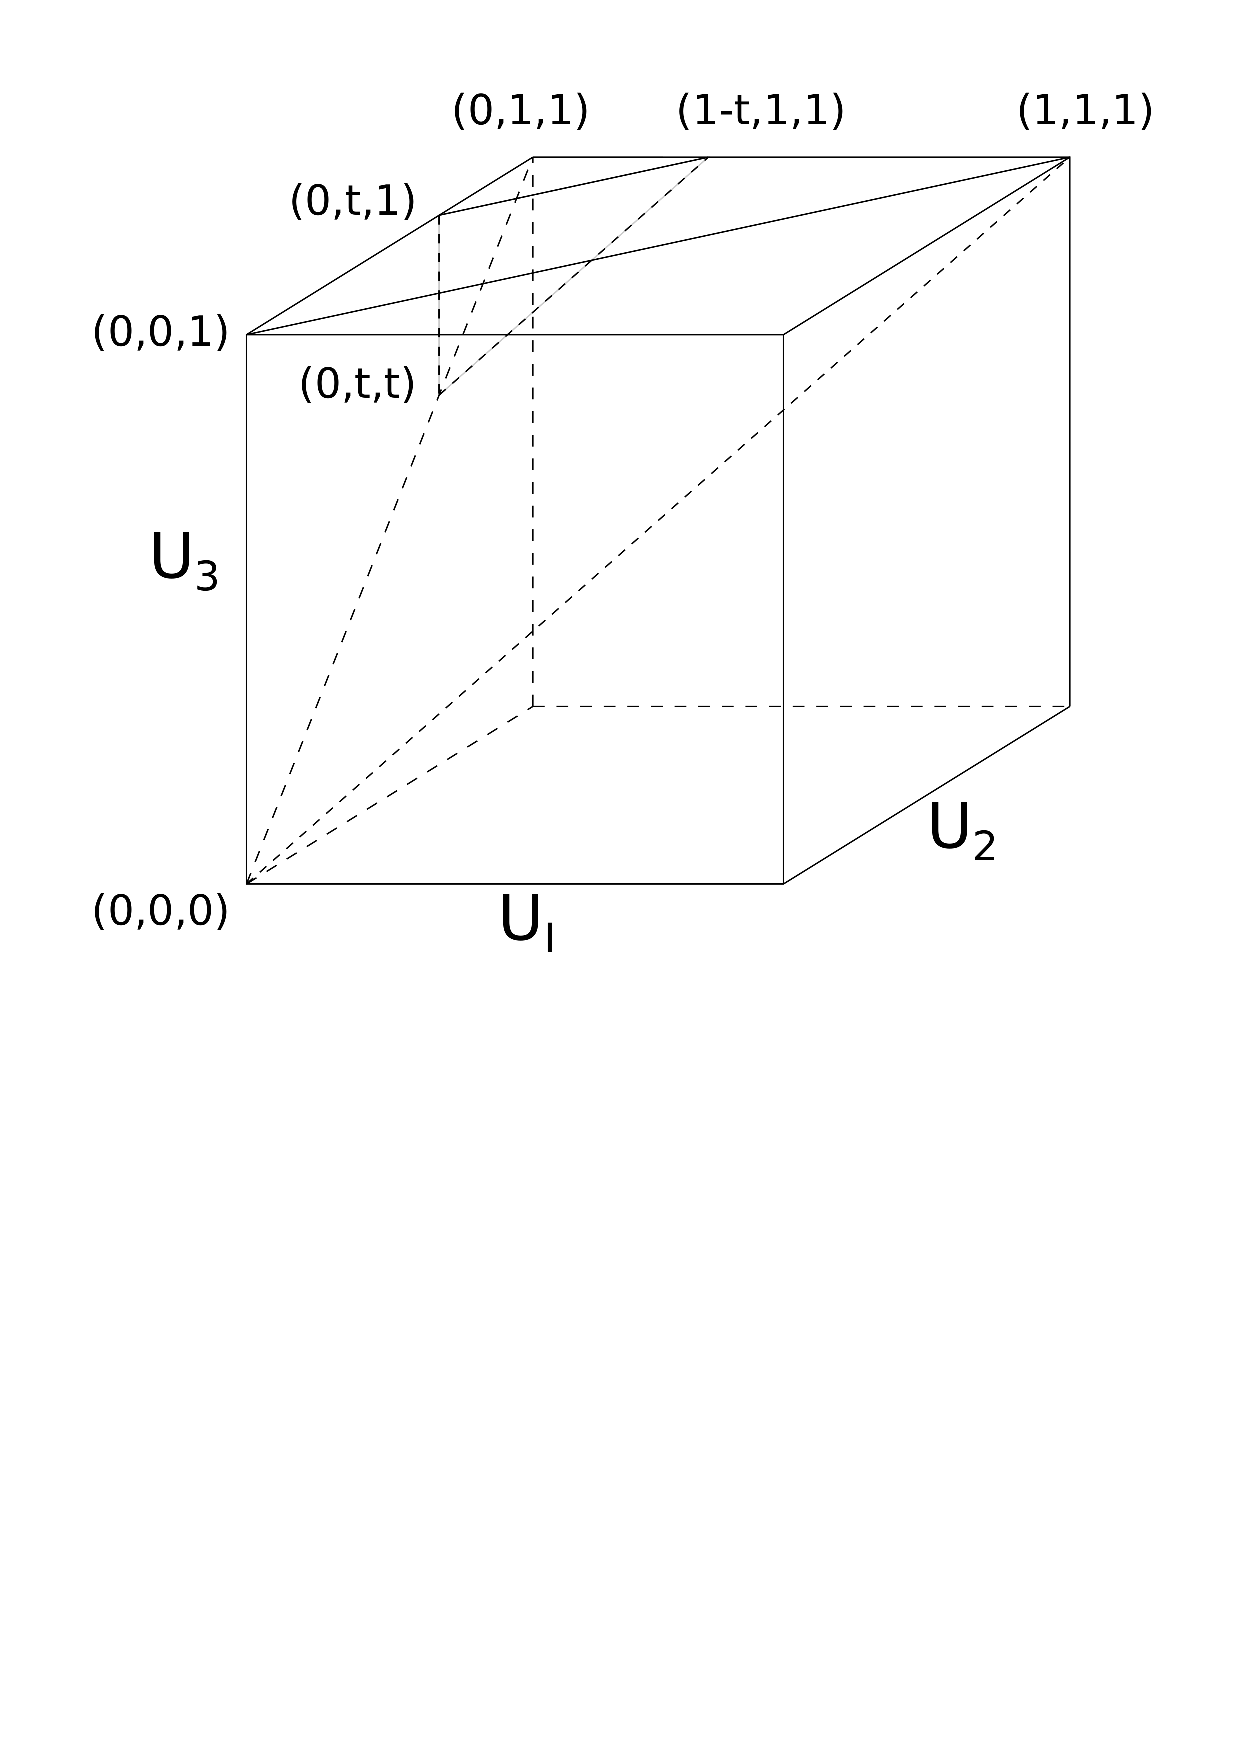
\includegraphics[scale=.5,trim=0 10cm 0 0, clip=true]{rank3d-nocolour}

The figure explains the probability estimation for the $n=3$ case. The rank statistics probability density is $3!=6$ and it uniformly scattered in (0,0,0), (0,0,1), (0,1,1), (1,1,1) tetrahedron. The $u_2 - u_1 \ge t$ condition holds only in the (0,t,t), (0,t,1), (0,1,1), (1-t,1,1) small tetrahedron.

To assess the p-value for a feature $i$, we do not need to rank the whole $r_{ij}, j=1..n$ vector to build the rank statistics $u_j$; we actually need only the $t$ value, so it is enough to find the maximal and the second values of $r_{ij}$.

\section{Discussion}

We formulated a statistical test that to detest reliable pairs of marker feature and the marked entity. Nevertheless the formulation of the problem looks abstract, its solution provides numerous straightforward application. The motivating example we started with was to detect the marker genes for expression patterns. The patterns could be obtained from the CoGAPS (scCoGAPS) \cite{Fertig_2016} or other matrix factorisation method \cite{Stein_2018}. The identification of the marker genes can critically simplify biological interpretation. If the matrix is the amplitude component from  the decomposition, the marker time points (or, the marker cells for scCoGAPS) can also be very informative for analysis. If the matrix contains the expression correlation for two gene sets, annotated best friends of an non-annotated gene extend the existing annotation.

\section{Conflict of interest}
The authors declare no conflict of interest.

\section{Acknowledgements}
AF acknowledges support by National Institutes of Health (NIH) P30CA006973 and 1U01CA253403-01, Russian Foundation for Basic Research (RFBR) 17-00-00208, the Russian Academy of Sciences Project 0112-2019-0001; VR acknowledges support from RFBR 20-54-12008; AM acknowledges support from RFBR 20-04-00459.

\bibliography{gene-best-friends}

\bibliographystyle{splncs03}
%\begin{subappendices}

\newcommand{\beginsupplement}{%
        \setcounter{table}{0}
        \renewcommand{\thetable}{S\arabic{table}}%
        \setcounter{figure}{0}
        \renewcommand{\thefigure}{S\arabic{figure}}
        \setcounter{equation}{0}
        \renewcommand{\theequation}{S\arabic{equation}}%
     }
\section*{Supplement}
\beginsupplement

%\renewcommand{\thesection}{\Alph{section}}%
% or try \arabic{section}
For an integer $m$,
\begin{eqnarray}
&\displaystyle \int_a^b\left(b-x\right)^{m-1}dx=
%-\displaystyle \int_0^{1-a}v^{n-1}dv=
\displaystyle \frac{\left(b-a\right)^m}{m}  \label{eq:intab}
\end{eqnarray} 
%\begin{eqnarray}
%&\displaystyle \int_a^1\left(1-x\right)^{m-1}dx=
%-\displaystyle \int_0^{1-a}v^{n-1}dv=
%\displaystyle \frac{\left(1-a\right)^m}{m}  \label{eq:right}
%\end{eqnarray} 
%\begin{eqnarray}
%&\displaystyle \int_0^b\left(b-x\right)^{m-1}dx=\displaystyle \frac{b^m}{m}  \label{eq:left}
%\end{eqnarray}
Applying \ref{eq:intab} recursively from $u_n$ until $u_1$: 
\begin{eqnarray}
V = &\displaystyle \int_0^1\int_{u_1}^1\int_{u_2}^1\int_{u_3}^1...\int_{u_{n-1}}^1 du_n...du_4 du_3 du_2 du_1 = \nonumber \\ 
&\displaystyle \frac{1}{(n-3)!}\int_0^1\int_{u_1}^1\int_{u_2}^1 \left( 1-u_3 \right)^{n-3}du_3 du_2 du_1 = \nonumber \\
&\displaystyle \frac{1}{(n-2)!}\int_0^{1-t}\int_{{u_1}+t}^1\left( 1-u_2 \right)^{n-2} du_2 du_1 = \nonumber \\
&\displaystyle \frac{1}{(n-1)!} \int_0^1\left( 1-u_1 \right)^{n-1} du_1 = \frac{1}{n!} \label{eq:volume}
\end{eqnarray} 
\begin{eqnarray}
& p_1(t) =  \displaystyle \frac{1}{V}\displaystyle \int_0^{1-t}\int_{{u_1}+t}^1\int_{u_2}^1\int_{u_3}^1...\int_{u_{n-1}}^1 du_n...du_2 du_1 =  \nonumber \\ 
%&\displaystyle \frac{n!}{(n-3)!}\int_0^{1-t}\int_{{u_1}+t}^1\int_{u_2}^1 \left( 1-u_3 \right)^{n-3}du_3 du_2 du_1 =  \nonumber \\
&\displaystyle \frac{n!}{(n-2)!}\int_0^{1-t}\int_{{u_1}+t}^1\left( 1-u_2 \right)^{n-2} du_2 du_1 =  \nonumber \\
&\displaystyle n \int_0^{1-t}\left( 1-t-u_1 \right)^{n-1} du_1 = (1-t)^n \label{eq:p_1}
\end{eqnarray}
\begin{eqnarray}
& p_k(t) = \displaystyle \frac{1}{V}\displaystyle \int_0^{1-t}\int_{{u_1}}^{1-t}...\int_{u_{k-1}}^{1-t}\int_{u_k+t}^1...\int_{u_{n-1}}^1 du_n... du_1 =  \nonumber \\ 
& \displaystyle \frac{n!}{(n-k-1)!}\displaystyle \int_0^{1-t}\int_{{u_1}}^{1-t}...\int_{u_{k-1}}^{1-t}\int_{u_k+t}^1 \left( 1-u_{k+1} \right)^{n-k-1} du_{k+1}...du_1 =  \nonumber \\
& \displaystyle \frac{n!}{(n-k)!}\displaystyle \int_0^{1-t}\int_{{u_1}}^{1-t}...\int_{u_{k-1}}^{1-t} \left( 1-t-u_{k} \right)^{n-k} du_k...du_1 =  \nonumber \\
& \displaystyle \frac{n!}{(n-k+1)!}\displaystyle \int_0^{1-t}\int_{{u_1}}^{1-t}...\int_{u_{k-2}}^{1-t} \left( 1-t-u_{k-1} \right)^{n-k+1} du_{k-1}...du_1 =  \nonumber \\
& \displaystyle n \int_0^{1-t}\left( 1-t-u_1 \right)^{n-1} du_1 = (1-t)^n \label{eq:p_k}
\end{eqnarray}
%\end{subappendices}
\begin{comment}
\subsection{ex-abstract}
Suppose we have set of {\tag}s $\T$ and a set of {\cloud}s $\C$ of this {\tag}s with some fuzzy membership, e.g. there is a numeric measure of how an {\tag} is represented in a {\cloud} $A(\tl,\cl)$ for each pair $(\tl,\cl):\tl \in \T, \cl \in \C$. The higher the $A(\tl,\cl)$ value is, the more the {\tag} $\tl$ is involved in the {\cloud} $\cl$. The absence of the {\tag} in the {\cloud} is shown by the value that is minimal for the {\cloud}.

An example that is easy to think about is: genes are {\tag}s and their groups under regulation by same transcription factors (TF’s) form {\cloud}s, and A shows the strength of the regulation. We look at a gene and we want to know whether a TF is its friend, i.e. whether the TF specifically prefers (regulates) the gene. The na\"ive idea is to look for a TF that the gene is the most sensitive for. Still, it’s possible that this TF is the strongest for the most of the genes. Sometimes, it is what we want to find, but now we want to answer other questions, namely, what TF is the most specific factor for the gene and is the specificity enough to say that is does not look like a random outcome?

Sometimes, the {\cloud}s are in in one-to-one relation with the {\tag}s, e.g. each {\cloud} is a set of {\tag}s, which are neighbours of {\tag} in some graph. For this example, A is a weighted adjacency matrix of this graph. The friendship terminology emerges naturally from this case. The friendship relation itself is asymmetric: a friend cares about Augustus, while Augustus does not.
\end{comment}
\end{document}


